\hypertarget{a00351}{}\section{Parameter update timing}
\label{a00351}\index{Parameter update timing@{Parameter update timing}}
Details about parameter timing and how to keep parameter updates in sync. 

\hypertarget{a00351_parameterUpdateTiming_contents}{}\subsection{On this page}\label{a00351_parameterUpdateTiming_contents}
\begin{DoxyItemize}
\item \hyperlink{a00351_parameterUpdateTiming_timelineLocations}{Timeline Locations} \item \hyperlink{a00351_parameterUpdateTiming_synchronization}{Coordinating the data model and algorithm} \item \hyperlink{a00351_parameterUpdateTiming_sharedData}{Fixing timing issues due to shared data} \item \hyperlink{a00351_parameterUpdateTiming_timestamps}{Determining the absolute timestamp for a parameter update}\end{DoxyItemize}
\hypertarget{a00351_parameterUpdateTiming_timelineLocations}{}\subsection{Timeline Locations}\label{a00351_parameterUpdateTiming_timelineLocations}
At any given moment, a plug-\/in may be asked to handle events from multiple locations on the timeline. Each module in an A\+A\+X plug-\/in may be updated using a different timeline position. For example\+: \begin{DoxyItemize}
\item During automation playback the host may choose to send parameter updates in advance, while the algorithm is still processing audio from earlier in the timeline. \item When a processing chain involves a significant amount of latency, the host may delay the metering data which is available to the plug-\/in\textquotesingle{}s G\+U\+I until the point in time when the corresponding processed audio is actually being played back to the user.\end{DoxyItemize}
In this article, we will refer to the following timeline locations\+: \begin{DoxyItemize}
\item {\itshape Automation time}\+: The location that corresponds to the state of the plug-\/in\textquotesingle{}s data model \item {\itshape Playhead}\+: The location where the audio engine is currently gathering samples for processing \item {\itshape Render time}\+: The location of the audio samples currently being processed by the plug-\/in\textquotesingle{}s algorithm \item {\itshape Presentation time}\+: The location that corresponds to the playback presentation to the user (i.\+e. the sound coming out of the speakers)\end{DoxyItemize}
 Figure 1\+: Timeline locations\hypertarget{a00351_parameterUpdateTiming_synchronization}{}\subsection{Coordinating the data model and algorithm}\label{a00351_parameterUpdateTiming_synchronization}
As an A\+A\+X plug-\/in developer, you don\textquotesingle{}t usually need to worry about the fact that your plug-\/in\textquotesingle{}s data model and algorithm may each represent a different point in the timeline; the \hyperlink{a00327_alg_comm}{A\+A\+X packet system} handles all of the necessary synchronization between these two locations.

This works seamlessly in a normal A\+A\+X plug-\/in because the real-\/time algorithm is fully decoupled from the plug-\/in\textquotesingle{}s data model. Since all of the state information for the algorithm is delivered through its \hyperlink{a00327_alg_memmgmt}{context structure}, the host can simply swap in the correct context data for each call to the processing callback. The plug-\/in does not require any special handling code to synchronize between the two timeline locations, and, as a bonus, A\+A\+X plug-\/ins can achieve deterministic, accurate automation playback without doing any extra work to handle time-\/stamped parameter update queues or other overhead.

 Figure 2\+: Synchronization through the A\+A\+X packet system\hypertarget{a00351_parameterUpdateTiming_packet_delivery}{}\subsubsection{A closer look at the A\+A\+X packet delivery system}\label{a00351_parameterUpdateTiming_packet_delivery}
\begin{DoxyParagraph}{Adding new packets for automation events}
When playing back automation, the A\+A\+X host calls \hyperlink{a00061_a685858711efb8634ce66c327f2865c71}{Update\+Parameter\+Normalized\+Value()} to update the data model state, then calls \hyperlink{a00061_a083265b008921b6114ede387711694b7}{Generate\+Coefficients()} to trigger the generation of new packets. See \hyperlink{a00353}{Basic parameter update sequences} for a full description of this sequence.

Before the host calls \hyperlink{a00061_a083265b008921b6114ede387711694b7}{Generate\+Coefficients()} to generate packets for an automation breakpoint, it records the timeline position of the breakpoint (\hyperlink{a00090_af9ab9b228023e116f89249a56c27a20f}{A\+A\+X\+\_\+\+I\+Controller\+::\+Get\+Current\+Automation\+Timestamp()} provides this value as a sample offset from the beginning of playback.) Every packet that is posted during execution of \hyperlink{a00061_a083265b008921b6114ede387711694b7}{Generate\+Coefficients()} is tagged with this timestamp when it is queued for delivery. 
\end{DoxyParagraph}


\begin{DoxyParagraph}{Packet delivery for A\+A\+X Native plug-\/ins}
As the playhead advances and sample buffers are queued for processing, the host tracks the location of the next time-\/stamped packet in the packet queue. As the render time location for a Native plug-\/in processing chain approaches the next packet time-\/stamp for a plug-\/in in the chain, the host divides the plug-\/in\textquotesingle{}s processing buffers into smaller buffers. When the render time location is as close as possible to the packet\textquotesingle{}s time-\/stamp, the host delivers the packet. The packet data is available to the algorithm in its context the next time it is executed.

Because the host may divide native processing buffers down to a minimum size of \hyperlink{a00206_aa1769ee466fd07659d8c7ef5ac61cd49a5819a4956c053084b094f686c920598e}{A\+A\+X\+\_\+e\+Audio\+Buffer\+Length\+Native\+\_\+\+Min} -\/ 32 samples -\/ the host can guarantee that all automation playback will be effected within 32 samples of the actual automation breakpoint location. In addition, with the help of some extra internal bookkeeping, A\+A\+X hosts also guarantee that the exact sample where an automation breakpoint is applied will be deterministic and will not change between different playback passes. 
\end{DoxyParagraph}


\begin{DoxyParagraph}{Packet delivery for A\+A\+X D\+S\+P plug-\/ins}
The packet delivery system for A\+A\+X D\+S\+P plug-\/ins works similarly to the system for A\+A\+X Native plug-\/ins. A\+A\+X D\+S\+P plug-\/ins use a fixed buffer size, so the host is not able to divide their playback buffers into smaller units\+: the plug-\/in will receive each data packet in the fixed-\/size playback buffer which most closely corresponds to the location of the automation event which triggered the packet.

An A\+A\+X D\+S\+P plug-\/in which declares an \hyperlink{a00283_a6571f4e41a5dd06e4067249228e2249ea09fbd1cbcae0e86ad81005258dc1b67e}{A\+A\+X\+\_\+e\+Property\+\_\+\+D\+S\+P\+\_\+\+Audio\+Buffer\+Length} value of N will be guaranteed to receive data packets within N/2 samples of the actual automation event position on the timeline. Since the default buffer size for an A\+A\+X D\+S\+P plug-\/in is 4 samples, this yields extremely accurate automation playback with no extra work required in the plug-\/in algorithm. 
\end{DoxyParagraph}
\hypertarget{a00351_parameterUpdateTiming_sharedData}{}\subsection{Fixing timing issues due to shared data}\label{a00351_parameterUpdateTiming_sharedData}
The packet system works perfectly to synchronize the states of the plug-\/in data model and algorithm, {\itshape but only when the plug-\/in algorithm is fully decoupled from the data model}. If the algorithm directly shares data with the data model then the algorithm will immediately start using any new data model state without waiting for the corresponding coefficient delivery.

Figure 3 shows one kind of problem that can arise when a plug-\/in uses the same state for both its data model and its algorithm. In this case, the plug-\/in applied a volume trim (shown in the automation lane at the top of the image) to its algorithm as soon as the parameter update was applied to its data model, even though the algorithm was not yet processing the audio at the Automation time location. As a result, the audio trim was applied several hundred samples too early.

 Figure 3\+: Offset automation playback due to lack of timeline location synchronization in a monolithic plug-\/in\hypertarget{a00351_parameterUpdateTiming_monolithic}{}\subsubsection{Monolithic plug-\/ins}\label{a00351_parameterUpdateTiming_monolithic}
Plug-\/ins that share data directly between their data model and algorithm are referred to as {\itshape monolithic}. All plug-\/ins that inherit from the \hyperlink{a00026}{A\+A\+X\+\_\+\+C\+Monolithic\+Parameters} helper class are monolithic.

\begin{DoxyNote}{Note}
Monolithic plug-\/ins must always set the \hyperlink{a00283_a6571f4e41a5dd06e4067249228e2249ea79a0815fea6c8f1a0d8ed511aa88e9ff}{A\+A\+X\+\_\+e\+Property\+\_\+\+Constraint\+\_\+\+Location} property to include \hyperlink{a00206_a0c5d795c1fd021c5b9b541febc34601aa027df08c137702400a92719828bea44b}{A\+A\+X\+\_\+e\+Constraint\+Location\+Mask\+\_\+\+Data\+Model} in order to avoid being loaded into incompatible A\+A\+X hosts.
\end{DoxyNote}
All monolithic plug-\/ins must include special handling code to reconcile the plug-\/in\textquotesingle{}s automation time state with its render time state.\hypertarget{a00351_parameterUpdateTiming_resolvingOffsets}{}\subsubsection{How to resolve timing errors}\label{a00351_parameterUpdateTiming_resolvingOffsets}
There are many possible solutions for the timing errors that arise when a plug-\/in combines data from different time locations. Ultimately, the plug-\/in must separate the state that is represented at different time locations.

In most cases, this requires deferring data model state changes from being applied to the algorithm until the relevant samples are being processed in the render callback. One easy way to accomplish this separation is to take advantage of the synchronization provided by the A\+A\+X packet delivery system. This approach benefits from the fact that it emulates the design of a normal, decoupled A\+A\+X plug-\/in.

After a packet is queued with a call to \hyperlink{a00090_ae5dd2b5925dbc181513bca1c4ac5e716}{Post\+Packet()}, the packet delivery system will wait to update the algorithm\textquotesingle{}s context structure with the packet\textquotesingle{}s data until the Render time location is very close to the automation event (see \hyperlink{a00351_parameterUpdateTiming_packet_delivery}{above}.) This provides an appropriate mechanism for deferring state changes in the plug-\/in\textquotesingle{}s data model until the Render time location has \char`\"{}caught up\char`\"{} to the correct sample.

Figure 4 shows the same scenario as Figure 3, but now the plug-\/in has been updated to defer data model updates from the automation time location so that they are applied as coefficients in the algorithm when the render time location has reached the correct point on the timeline.

 Figure 4\+: Deferring a data model update in a monolithic plug-\/in using the packet queue

Here is one way to use the packet delivery system to defer changes to the data model state\+: 
\begin{DoxyCode}
\hyperlink{a00149_a4d8f69a697df7f70c3a8e9b8ee130d2f}{AAX\_Result}
MyEffectParameters::UpdateParameterNormalizedValue(
  \hyperlink{a00149_a1440c756fe5cb158b78193b2fc1780d1}{AAX\_CParamID} iParamID,
  \textcolor{keywordtype}{double} aValue,
  \hyperlink{a00206_a30be0398faf20c6b121239eb9399f3f7}{AAX\_EUpdateSource} inSource)
\{
  \textcolor{comment}{// Call inherited}
  \hyperlink{a00149_a4d8f69a697df7f70c3a8e9b8ee130d2f}{AAX\_Result} result = 
      \hyperlink{a00026_a2ebeb6e1cc24277c7e72abbbfbebb5e9}{AAX\_CMonolithicParameters::UpdateParameterNormalizedValue}
      (
    iParamID,
    aValue,
    inSource);
  \textcolor{keywordflow}{if} (\hyperlink{a00207_a5f8c7439f3a706c4f8315a9609811937aeddbd1bb67e3a66e6af54a4b4a7a57b3}{AAX\_SUCCESS} != result) \{ \textcolor{keywordflow}{return} result; \}
  
  \textcolor{comment}{// Do whatever additional work is required to note that the}
  \textcolor{comment}{// parameter has been updated - for example, set a "dirty"}
  \textcolor{comment}{// flag for the parameter.}
  
  \textcolor{keywordflow}{return} result;
\}
\end{DoxyCode}



\begin{DoxyCode}
\hyperlink{a00149_a4d8f69a697df7f70c3a8e9b8ee130d2f}{AAX\_Result}
MyEffectParameters::GenerateCoefficients()
\{
  \textcolor{comment}{// Call inherited}
  \hyperlink{a00149_a4d8f69a697df7f70c3a8e9b8ee130d2f}{AAX\_Result} result = \hyperlink{a00026_ac9a3a7ac90562135ceb4b80301e12e92}{AAX\_CMonolithicParameters::GenerateCoefficients}
      ();
  \textcolor{keywordflow}{if} (\hyperlink{a00207_a5f8c7439f3a706c4f8315a9609811937aeddbd1bb67e3a66e6af54a4b4a7a57b3}{AAX\_SUCCESS} != result) \{ \textcolor{keywordflow}{return} result; \}
  
  \textcolor{keyword}{const} uint32\_t stateNum = mMyStateCounter++; \textcolor{comment}{// member uint32\_t}
  
  \textcolor{comment}{// Do whatever additional work is required to capture the current}
  \textcolor{comment}{// parameter state and associate it with stateNum, for example}
  \textcolor{comment}{// check for "dirty" parameters and create a list of these}
  \textcolor{comment}{// parameters with their values, add this list to a map using}
  \textcolor{comment}{// stateNum as a key, and clear the "dirty" flags.}
  
  result = Controller()->PostPacket(
    kCurrentStateFieldIndex,
    &stateNum,
    \textcolor{keyword}{sizeof}(uint32\_t));
   
  \textcolor{keywordflow}{return} result;
\}
\end{DoxyCode}



\begin{DoxyCode}
\textcolor{keyword}{struct }MyContextStructure
\{
  int32\_t * mCurrentStateNum; \textcolor{comment}{// Private data}
  \textcolor{comment}{// ...}
\};

\textcolor{keywordtype}{void}
MyAudioRenderCallback(
  MyContextStructure* \textcolor{keyword}{const} inInstancesBegin [],
  \textcolor{keyword}{const} \textcolor{keywordtype}{void}* inInstancesEnd)
\{
  \textcolor{comment}{/* For each instance... */}
  \textcolor{keyword}{const} uint32\_t stateNum = instance->mCurrentStateNum;
  
  \textcolor{comment}{// Update the custom plug-in object state based on stateNum}
  \textcolor{comment}{// and the additional data that was cached during}
  \textcolor{comment}{// GenerateCoefficients().}
\}   
\end{DoxyCode}


 Figure 5\+: One specific solution for deferring a data model update in a monolithic plug-\/in using the packet queue

This approach is incorporated directly into the design of \hyperlink{a00026}{A\+A\+X\+\_\+\+C\+Monolithic\+Parameters}. If your plug-\/in data model is a subclass of \hyperlink{a00026}{A\+A\+X\+\_\+\+C\+Monolithic\+Parameters} then you can follow these steps to ensure accurate parameter update timing in your plug-\/in\+:


\begin{DoxyEnumerate}
\item After creating an automatable parameter, call \hyperlink{a00026_a1b23573e8aa3f8e64c61813b721559c2}{A\+A\+X\+\_\+\+C\+Monolithic\+Parameters\+::\+Add\+Synchronized\+Parameter()} to add the parameter to an internal list of parameters to synchronize using the deferred-\/update system  
\item In the plug-\/in\textquotesingle{}s \hyperlink{a00026_a04f2f73d70ea28c17747c68fc3a20fc8}{Render\+Audio()} implementation, iterate through the incoming queue of deferred parameter values  
\item Update the coefficients used by the plug-\/in\textquotesingle{}s algorithm or other processing components  
\end{DoxyEnumerate}

N\+O\+T\+E\+S 
\begin{DoxyItemize}
\item Remember to use the deferred parameter values, not values of the plug-\/in\textquotesingle{}s \hyperlink{a00108}{A\+A\+X\+\_\+\+I\+Parameter} objects, when setting the state of the plug-\/in\textquotesingle{}s coefficients  
\item The deferred parameter values are delivered in the real-\/time thread, so all synchronized updates should follow the basic principles of real-\/time operation such as avoiding memory allocation/free, thread synchronization, access to shared resources, or any other actions which could block the real-\/time thread  
\end{DoxyItemize}

For reference, see \hyperlink{a00376_DemoMIDI_Synth}{Demo\+M\+I\+D\+I\+\_\+\+Synth} and the other example instrument plug-\/ins. All of the instrument examples in the A\+A\+X S\+D\+K use these facilities to achieve deterministic, accurate playback for automated parameters.

One benefit of this approach is that it provides a compatible interface with monolithic plug-\/in objects which are designed to work across multiple plug-\/in formats. For example, the set of parameter updates provided to \hyperlink{a00026_a04f2f73d70ea28c17747c68fc3a20fc8}{A\+A\+X\+\_\+\+C\+Monolithic\+Parameters\+::\+Render\+Audio()} \char`\"{}\+Render\+Audio\char`\"{} can be provided to plug-\/in objects which require a queue of time-\/stamped parameter updates for each audio render callback.\hypertarget{a00351_parameterUpdateTiming_considerations}{}\subsubsection{Additional considerations}\label{a00351_parameterUpdateTiming_considerations}
Of course, the approach described in this section is just one possible solution. The \hyperlink{a00351_parameterUpdateTiming_timestamps}{timestamp} section below provides some alternatives to using the packet queue system for synchronization. Ultimately, the best design for your plug-\/in will depend on the facilities that are available in the plug-\/in\textquotesingle{}s monolithic state object, the size of this object, its interface, the number of parameters representing its state, and other internal details.

Here are some additional factors to consider when using the packet queue system for time location synchronization of parameter updates\+: \begin{DoxyItemize}
\item The algorithm callback / \hyperlink{a00026_a04f2f73d70ea28c17747c68fc3a20fc8}{Render\+Audio()} method is called from a real-\/time thread, and may be called concurrently with data model methods. You should use a synchronization strategy that is optimized for high performance in this thread. \item If a parameter is not automatable then you should probably ignore these additional steps and directly update the plug-\/in\textquotesingle{}s monolithic state object from within \hyperlink{a00061_a685858711efb8634ce66c327f2865c71}{Update\+Parameter\+Normalized\+Value()} when that parameter is changed. Updates for non-\/automatable parameters can always be applied to the algorithm \char`\"{}as soon as possible\char`\"{}. \item Depending on your plug-\/in\textquotesingle{}s design you may not need or want to apply this solution to some automatable parameters either. For example, parameters that are unlikely to be automated or which require C\+P\+U-\/intensive changes in your instrument object should probably be updated on the object directly from within \hyperlink{a00061_a685858711efb8634ce66c327f2865c71}{Update\+Parameter\+Normalized\+Value()}, and not from within the real-\/time thread\end{DoxyItemize}
\hypertarget{a00351_parameterUpdateTiming_timestamps}{}\subsection{Determining the absolute timestamp for a parameter update}\label{a00351_parameterUpdateTiming_timestamps}
The A\+A\+X packet queue provides a host-\/managed system for applying parameter updates at the correct location without requiring any special knowledge about the timeline. However, In some situations a plug-\/in may need to know the absolute sample position of a parameter change.

For example, a plug-\/in that synchronizes parameter changes to some external system, and which wants to forward these changes over to the external system as early as possible, would want to know the sample position for a coefficient update when the update is first triggered by a call to \hyperlink{a00061_a083265b008921b6114ede387711694b7}{Generate\+Coefficients}.

In these situations it is not suitable to simply use a method like \hyperlink{a00116_a8119233b03774528ffaa519771d792a0}{A\+A\+X\+\_\+\+I\+Transport\+::\+Get\+Current\+Native\+Sample\+Location()} which returns the current position of the audio render thread. The parameter update may be occurring at a different location on the timeline from the current render position, so using the current render position for the update would result in timeline offset problems similar to those described above.\hypertarget{a00351_parameterUpdateTiming_timelineMethods}{}\subsubsection{Obtaining timeline information}\label{a00351_parameterUpdateTiming_timelineMethods}
A\+A\+X provides a variety of information that can be used for timeline synchronization. This information is provided through a combination of \hyperlink{a00116}{A\+A\+X\+\_\+\+I\+Transport}, \hyperlink{a00090}{A\+A\+X\+\_\+\+I\+Controller}, and M\+I\+D\+I beat clock data. Here is a summary of the relevant ways that a plug-\/in can get information about the timeline and timing synchronization data\+:


\begin{DoxyItemize}
\item \hyperlink{a00116_a8119233b03774528ffaa519771d792a0}{A\+A\+X\+\_\+\+I\+Transport\+::\+Get\+Current\+Native\+Sample\+Location()}  Provides the absolute sample position of the first sample in the audio buffer that is currently being processed by the plug-\/in\textquotesingle{}s worker chain   
\item \hyperlink{a00090_afbc2973d755b6c3ae82b6c8461e9fdee}{A\+A\+X\+\_\+\+I\+Controller\+::\+Get\+T\+O\+D\+Location()}  Provides the current \char`\"{}time of day\char`\"{} value, which is a counter within the audio engine that counts the number of samples that the playhead has traversed since playback start   
\item \hyperlink{a00090_af9ab9b228023e116f89249a56c27a20f}{A\+A\+X\+\_\+\+I\+Controller\+::\+Get\+Current\+Automation\+Timestamp()}  Must be called from within \hyperlink{a00061_a083265b008921b6114ede387711694b7}{Generate\+Coefficients}. Provides the timestamp for the beginning of the hardware audio buffer during which the generated coefficients will be applied to the algorithm. This timestamp is provided in terms of the \char`\"{}time of day\char`\"{} counter, i.\+e. the number of samples since playback started.   
\item M\+I\+D\+I Beat Clock  Sends transport start/continue/stop events to plug-\/ins that register global M\+I\+D\+I nodes   
\end{DoxyItemize}\hypertarget{a00351_parameterUpdateTiming_determiningTimelinePosition}{}\subsubsection{Determining the timeline position of a parameter update}\label{a00351_parameterUpdateTiming_determiningTimelinePosition}
Each of the available methods for getting information about the timeline position has a particular purpose. No single interface method can be used to directly determine the sample location for a parameter update, but it is possible to determine this value by combining information from a few of the available methods.

Here are some possible approaches for determining the timeline position of a parameter update

\begin{DoxyNote}{Note}
Remember that these are not strict recipes; the specific requirements for what kinds of timeline information are needed will vary from plug-\/in to plug-\/in. You may be able to refine these approach to better match the needs of your specific plug-\/in.
\end{DoxyNote}
\hypertarget{a00351_parameterUpdateTiming_determiningTimelinePosition_1}{}\paragraph{1. Defer the update to the real-\/time thread}\label{a00351_parameterUpdateTiming_determiningTimelinePosition_1}

\begin{DoxyEnumerate}
\item Queue state updates using a plug-\/in design similar to the one described \hyperlink{a00351_parameterUpdateTiming_resolvingOffsets}{above}  
\item When a state update is received on the real-\/time thread, call \hyperlink{a00116_a8119233b03774528ffaa519771d792a0}{Get\+Current\+Native\+Sample\+Location} to get the sample location for the start of the current render buffer  
\item Perform all necessary update handling using this value as the sample location  
\end{DoxyEnumerate}

N\+O\+T\+E\+S \begin{DoxyItemize}
\item This approach yields a sample location value which is accurate within 32 samples \item Event handling must be performed on the real-\/time render thread, which may not be viable depending on the types of operations that the plug-\/in must perform \item Event handling cannot be performed in advance to reduce overall system latency\end{DoxyItemize}
\hypertarget{a00351_parameterUpdateTiming_determiningTimelinePosition_2}{}\paragraph{2. Compute the timestamp as a T\+O\+D offset}\label{a00351_parameterUpdateTiming_determiningTimelinePosition_2}

\begin{DoxyEnumerate}
\item Add a queue for update events which will be used internally within the plug-\/in\textquotesingle{}s \hyperlink{a00099}{A\+A\+X\+\_\+\+I\+Effect\+Parameters} object  
\item In \hyperlink{a00061_a685858711efb8634ce66c327f2865c71}{Update\+Parameter\+Normalized\+Value}, enqueue an update event  
\item In \hyperlink{a00061_a083265b008921b6114ede387711694b7}{Generate\+Coefficients}, call \hyperlink{a00090_afbc2973d755b6c3ae82b6c8461e9fdee}{A\+A\+X\+\_\+\+I\+Controller\+::\+Get\+T\+O\+D\+Location()} and \hyperlink{a00090_af9ab9b228023e116f89249a56c27a20f}{A\+A\+X\+\_\+\+I\+Controller\+::\+Get\+Current\+Automation\+Timestamp()}  
\item Subtract the current T\+O\+D value from the automation timestamp to find the number of samples currently lie between the data model location and the render audio location on the timeline  
\item Call \hyperlink{a00116_a8119233b03774528ffaa519771d792a0}{A\+A\+X\+\_\+\+I\+Transport\+::\+Get\+Current\+Native\+Sample\+Location()} and add the resulting value to the sample offset that was determined in the last step. The sum of these two values is the approximate absolute sample location for the coefficient update.  
\item Once this sample location has been calculated, dequeue all pending update events and handle them using the calculated timestamp  
\end{DoxyEnumerate}

The reason that this approach yields an approximate value is that the T\+O\+D location and current playback location are both given in terms of the real-\/time audio workers, and these values continue to progress simultaneously with execution of methods on the automation update thread. As a result, this approach will yield an absolute timestamp that is \char`\"{}late\char`\"{} by between zero and one hardware buffer.

N\+O\+T\+E\+S \begin{DoxyItemize}
\item Using this approach it is possible to handle parameter updates in advance to reduce overall system latency \item This approach yields a sample location value which is accurate within one hardware buffer \item This approach uses A\+A\+X interface methods that are not supported in older A\+A\+X hosts such as Pro Tools 10\end{DoxyItemize}
\hypertarget{a00351_parameterUpdateTiming_determiningTimelinePosition_3}{}\paragraph{3. Compute the timestamp with improved accuracy using M\+I\+D\+I Beat Clock}\label{a00351_parameterUpdateTiming_determiningTimelinePosition_3}
You can refine the approach described above by using M\+B\+C events to detect the location of playback start.


\begin{DoxyEnumerate}
\item Register a global M\+I\+D\+I node in your plug-\/in using \hyperlink{a00096_aa7709de005e0256feb522758ccc5b582}{A\+A\+X\+\_\+\+I\+Effect\+Descriptor\+::\+Add\+Control\+M\+I\+D\+I\+Node()} with \hyperlink{a00206_a5e1dffce35d05990dbbad651702678e4a2be91828f8c1dac20ab5dff136fc1fce}{A\+A\+X\+\_\+e\+M\+I\+D\+I\+Node\+Type\+\_\+\+Global} and the appropriate event mask bitfield for M\+B\+C events  
\item Override \hyperlink{a00062_ab4ec161f64086070083c21b566354861}{A\+A\+X\+\_\+\+I\+Effect\+Parameters\+::\+Update\+Control\+M\+I\+D\+I\+Nodes()} to receive M\+B\+C data  
\item When an M\+B\+C Start or Continue event is received, call \hyperlink{a00116_a8119233b03774528ffaa519771d792a0}{A\+A\+X\+\_\+\+I\+Transport\+::\+Get\+Current\+Native\+Sample\+Location()} to get the current render location. Cache this value. This value should represent the absolute playback start sample since audio render will not have started before the M\+B\+C event dispatch.  
\item As in the previous solution, queue relevant update events in \hyperlink{a00061_a685858711efb8634ce66c327f2865c71}{Update\+Parameter\+Normalized\+Value}  
\item In \hyperlink{a00061_a083265b008921b6114ede387711694b7}{Generate\+Coefficients}, call \hyperlink{a00090_af9ab9b228023e116f89249a56c27a20f}{Get\+Current\+Automation\+Timestamp} and add the resulting value to the cached playback start sample location  
\item Dequeue all pending update events and handle them using the calculated absolute sample timestamp  
\end{DoxyEnumerate}

N\+O\+T\+E\+S \begin{DoxyItemize}
\item Using this approach it is possible to handle parameter updates in advance to reduce overall system latency \item This approach will yield timestamps within a few samples of the actual automation event location on the Pro Tools timeline \item This approach uses A\+A\+X interface methods that are not supported in older A\+A\+X hosts such as Pro Tools 10 \end{DoxyItemize}
Collaboration diagram for Parameter update timing\+:
\nopagebreak
\begin{figure}[H]
\begin{center}
\leavevmode
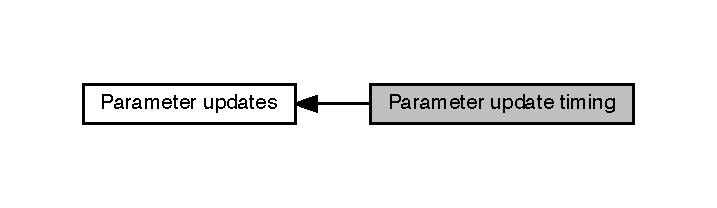
\includegraphics[width=344pt]{a00351}
\end{center}
\end{figure}
